%!TEX root = p.tex
\section{Explorer 2}
User testing revealed several shortcomings in first version of the ``Explorer" interface. In the second iteration, we sought to address all of these. In this section, we discuss each major piece of feedback and the changes we made in response.

\begin{figure}[htb]
  \centerline{
    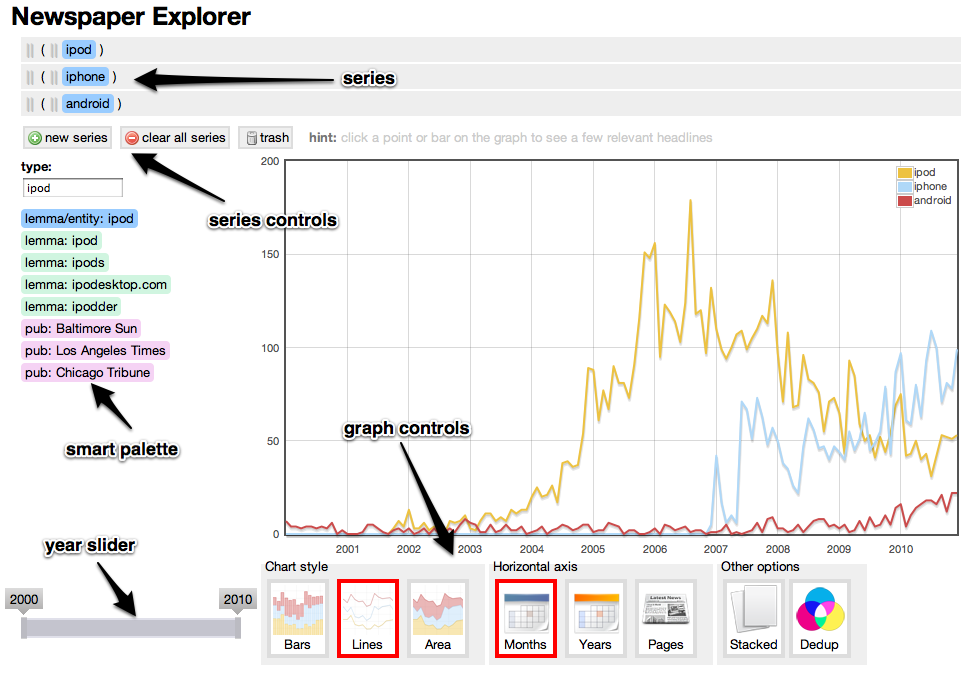
\includegraphics[scale=0.25]{figures/explorer-ui.png}
  }
  \caption{Second iteration of Explorer interface}
  \label{fig:explorer-ui}
\end{figure}

\textbf{The interactions required for creating series were very cumbersome and limiting series to disjunctions was too limiting for expressiveness.} In order to make series more expressive, we now allow arbitrary conjunctive normal form expressions to be used for series. Additionally, we introduced a type system for terms, with support for Publication, Entity, Lemma, Page, and Sentiment types. This allows for the specification of complex queries like ``first page articles mentioning New York in the Baltimore Sun or Los Angeles Times" (see figure).
To make constructing and modifying expressions more intuitive, we implemented a drag and drop, touch-friendly interface. Terms and disjunctive clauses can be dragged within and between series. Series can be created by clicking the New Series button or by dropping a term or clause onto it. In the latter case, the new series will be pre-populated with the dropped clause or with a new clause containing the dropped term. Similarly, dropping a term on an existing series but outside an existing clause will create a new clause containing that term. Finally, terms, clauses, and entire series can be dragged and dropped onto the Trash box, which will result in their deletion. 

\begin{figure}[htb]
  \centerline{
    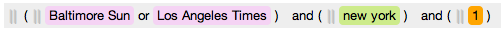
\includegraphics[scale=0.28]{figures/builder-series.png}
  }
  \caption{A complex expression demonstrating the use of conjunctive normal formed and typed terms}
  \label{fig:builder-series}
\end{figure}


Terms originate in the ``smart palette" sidebar on the left of the screen. The user types a term in the input box, and has the option to use a lemma/entity term containing the exact text they typed or to choose from a number of auto-complete suggestions that appear below. When possible, the suggested terms are annotated with icons representing the data class (we currently support people, places, and organizations). Terms for the three publications are also available in the palette, and page number terms become available when the user types a number.

\begin{figure}[htb]
  \centerline{
    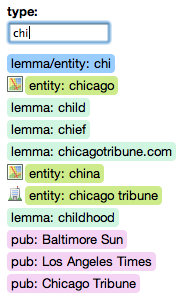
\includegraphics[scale=0.28]{figures/smart-palette.png}
  }
  \caption{Smart palette sidebar populated with typed suggestions}
  \label{fig:smart-palette}
\end{figure}


\textbf{Users were confused about what exactly the filter functionality did.} In light of this feedback as well as the increased expressiveness of the series functionality, we decided to remove the global filter in this iteration.

\textbf{Testers wanted the ability to figure out why spikes occurred in series.} In user testing, we found that even in its first iteration, the Explorer tool was fairly effective for finding interesting features in time series. However, our testers expressed frustration when we explained that there was no way to figure out why these features occurred. Part of this had to do with our usage license for the data, which prohibits us from exposing the full-text of the articles. To work around this issue we added the ``headline inspector" view, a floating dismissible window that shows up to 20 headlines from the most recently clicked point on the graph. Empirically, we found that scanning the headlines was usually sufficient for testers to identify the cause of a spike.


\begin{figure}[htb]
  \centerline{
    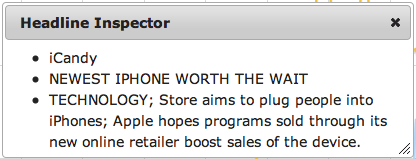
\includegraphics[scale=0.28]{figures/details.png}
  }
  \caption{Headline inspector window}
  \label{fig:details}
\end{figure}



\textbf{The graph controls were unappealing and hard to decode.} Specifically, our users indicated that it was difficult to quickly change the various graph settings. We replaced the complex drop downs and radio buttons with large buttons with icons representing their function. This had the added benefit of making these controls more touch-friendly.

\textbf{The interface did not allow for sharing and collaboration.} To remedy this issue, we made the URL update to reflect the state of the graph interface, to allow for sharing of interesting graphs by copying and pasting the contents of the browser address bar. This is the most familiar way of sharing for many users and is also most compatible with various browser plugins used for sharing.

